\subsection{Motivation}

First introduced by Ying and coworkers \cite{Ying:2004:JCP}, the kernel-independent FMM
provides an algorithm, that maintains the basic recursive structure and $O(N)$
asymptotic complexity of the analytic FMM, but without the requirement for the
implementation of analytic expansions of the kernel function for each kernel.
Instead the method relies only on kernel function evaluations. This allows
software implementations to be written in an easily extensible manner for different
kernels. The main difference to the analytic FMM of Section \ref{sec:1_1_fmm_overview},
lie in the the way that source and target densities are represented, and how
the M2M, L2L and M2L operators are computed.

For the kernel-independent FMM the \gls{far-field}, $\mathcal{F}^B$, and
\gls{near-field}, $\mathcal{N}^B$, are specified precisely. For a given box $B$
centered at $\mathbf{c}$ with sides of length 2$r$, $\mathcal{N}^B$ is a box
centered at $\mathbf{c}$ with sides of length 6$r$. The \gls{far-field} is then
$\mathbb{R}^d / \mathcal{N}^B$. Here, $B$ is in the \gls{near-field}. Now,
consider the potential in the \gls{far-field} $\mathcal{F}^B$, generated by a
set of \gls{source-particles} with \textbf{\gls{source-densities}}

The introduction of this algorithm requires the concepts of \textit{equivalent densities}
and \textit{check surfaces}.


\begin{figure}[!h]
    \centering
    {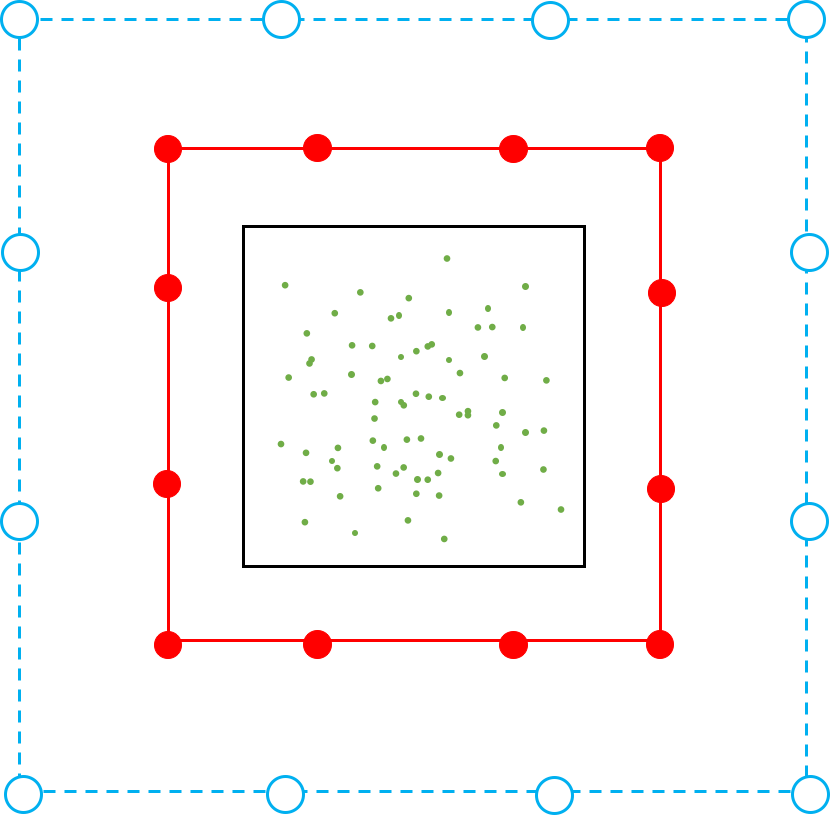
\includegraphics[width=0.3\textwidth]{introduction/upward_surface.png}}
    \hfill
  {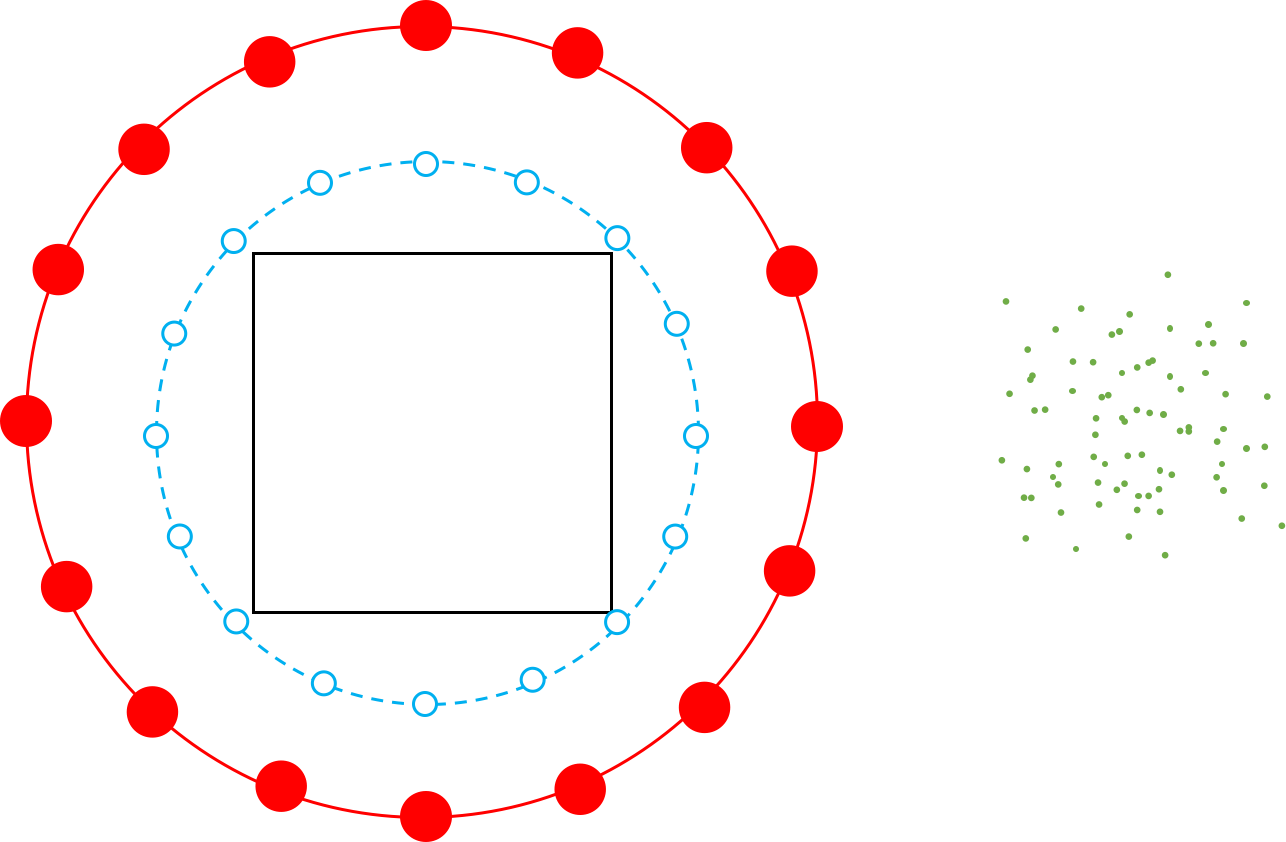
\includegraphics[width=0.4\textwidth]{introduction/downward_surface.png}}
  \vspace{0pt}
  \caption{Foo Bar}

  \label{fig:1_2_upward_downward_surfaces}
\end{figure}

\subsection{Algorithm Structure \& Analysis}


\subsection{Summary}

